\documentclass[11pt]{article}
\usepackage[letterpaper,margin=1in]{geometry}
\usepackage{color}
\usepackage[dvipdfmx]{graphicx}
\usepackage{amsbsy}
\usepackage{amssymb}
\usepackage{amsmath}
\usepackage{adjustbox}
\usepackage{url}
\usepackage{mathtools}
\DeclarePairedDelimiter\ceil{\lceil}{\rceil}
\DeclarePairedDelimiter\floor{\lfloor}{\rfloor}

\newcommand{\argmax}{\mathop{\rm arg~max}\limits}
\newenvironment{claim}[1]{\par\noindent\underline{Claim:}\space#1}{}
\newenvironment{claimproof}[1]{\par\noindent\underline{Proof:}\space#1}{\hfill $\blacksquare$}


\begin{document}
\title{Analysis Report on Assignment 5: PAC Learnability}
\author{Yoshinari Fujinuma}
\date{}
\maketitle

\section{Problem 1}
% http://grandmaster.colorado.edu/~cketelsen/files/csci5622/videos/lesson12/lesson12.pdf
``any consistent learner using $H=C$ will, with probability $95\%$, output a hypothesis with error at most $0.15$''

error $\epsilon = 0.15$

confidence $\delta = 0.05$

What is the number of sufficient training data size $m$?

Since class $C$ is finite, the hypothesis $H$ is also finite.

The number of hypothesis $|H|$ is any combinations of three different points:
$$
|H| = \dbinom{N}{3} = 161700
$$
where $N$ is the number of points in $[0, 99]$. So $N = 100$.

According to Lecture 12\footnote{http://grandmaster.colorado.edu/~cketelsen/files/csci5622/videos/lesson12/lesson12.pdf}, the concept $c$ is PAC learnable with 
$$
m \geq \frac{1}{\epsilon}(\log |H| + \log(\frac{1}{\delta}))
$$
By plugging in $\epsilon = 0.15$ and $\delta = 0.05$, 
$$
m \geq \frac{1}{0.15}(\log(161700) + \log(\frac{1}{0.05})) \approx 99.928
$$
So the bound or the minimum number of training examples necessary is $m = \ceil{99.928} = 100$.


\section{Problem 2}
``State and prove the VC Dimension of the hypothesis class H of linear hyperplanes in 2D that pass through the origin.''

According to Lecture 13\footnote{http://grandmaster.colorado.edu/~cketelsen/files/csci5622/videos/lesson13/lesson13.pdf}, the VC dimension is defined as the following:
$$
\mbox{VCdim}(H) = max{|S|: H \mbox{ shatters } S \mbox{ for some } S}
$$

Decision boundary: 
$$ 
h(x, y) = \begin{cases} 
          +1 \mbox{ if } ax - y \geq 0 \mbox{ (i.e. above the line) }\\
          -1 \mbox{ if } ax - y < 0 \mbox{ (i.e. below the line) }\\
\end{cases}
$$


E.g., For a point ()

\subsection{Proof of the lower bound}

For a given $2$ points in 2D, we can shatter in similar way to slides 22 through 25.

\begin{figure}[htb]
  \begin{center}
   \begin{tabular}{c}
    \begin{minipage}{0.5\hsize}
     \begin{center}
     \scalebox{0.33}
      {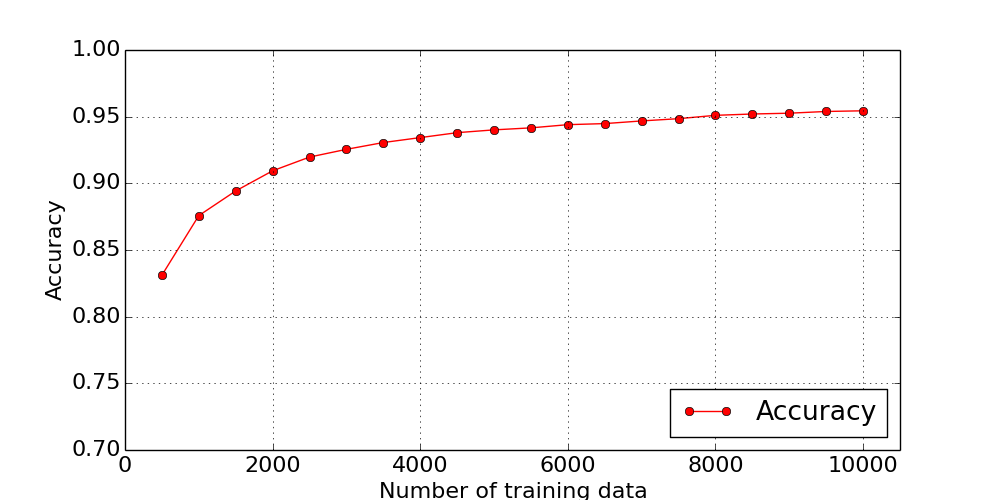
\includegraphics[]{figure_1.png}}
   
      \caption{$a = 4/5$. }
      \label{fig:corpus_size}
     \end{center}
    \end{minipage}

    \begin{minipage}{0.01\hsize}
    \end{minipage}

%    \begin{minipage}{0.5\hsize}
%     \begin{center}
%      \scalebox{0.33}
%      {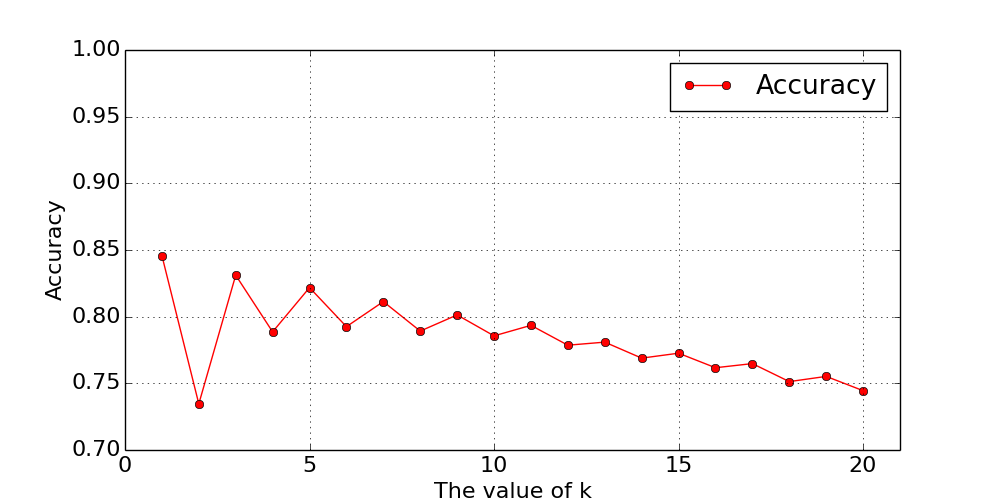
\includegraphics[]{figure_2.png}}
%      \caption{\label{k_and_accuracy}The relationship between $k$ and accuracy. The value of the number of training examples is fixed to $500$}
%     \end{center}
%    \end{minipage}

  \end{tabular}
 \end{center}
\end{figure}

So $\mbox{VCdim}(H) \geq 2$.

\subsection{Proof of the upper bound}

\begin{claim}
$$\mbox{VCdim}(H) < 3.$$
\end{claim}

\begin{claimproof}
We will prove by contradiction.

Let given three points $(x_1, y_1)$, $(x_2, y_2)$, $(x_3, y_3)$ have labels ${l_1 = +1, l_2 = -1, l_3 = +1}$ respectively.

Assume $0 \leq x_1 < x_2 < x_3$ and $y_1 > y_2 > y_3 \geq 0$.

Since $l_1 = +1$, $ax_1 - y_1 \leq 0$

Since $l_3 = +1$, $ax_3 - y_3 \leq 0$

From the assumption, and assuming $a > 0$ (i.e. only considering the first quadrant), $$ax_1 < ax_2 < ax_3$$. 

Since $y_1, y_2, y_3 \geq 0$, $$ax_1 - y_1 < ax_2 - y_1 < ax_3 - y_1$$.

Since $y_1 > y_2 > y_3 \geq 0$, $$ax_1 - y_1 < ax_2 - y_2 < ax_3 - y_3 \leq 0$$.

Therefore,$$ax_2 - y_2 \leq 0.$$
However, this contradicts to the assumption that $l_2 = -1$, i.e. $ax_2 - y_2 > 0$.
\end{claimproof}

\end{document}

